\documentclass{article}

\usepackage{graphicx}
\usepackage{tikz}
\usepackage{tikzsymbols}
\usetikzlibrary{calc,patterns,shapes.geometric}
\pagestyle{empty}
\usepackage[margin=0pt]{geometry}
\geometry{papersize={14in,12in}}

\def\centerarc[#1](#2)(#3:#4:#5){\draw[#1] ($(#2)+({#5*cos(#3)},{#5*sin(#3)})$) arc (#3:#4:#5);}

\begin{document}
	\begin{figure}
		\centering
		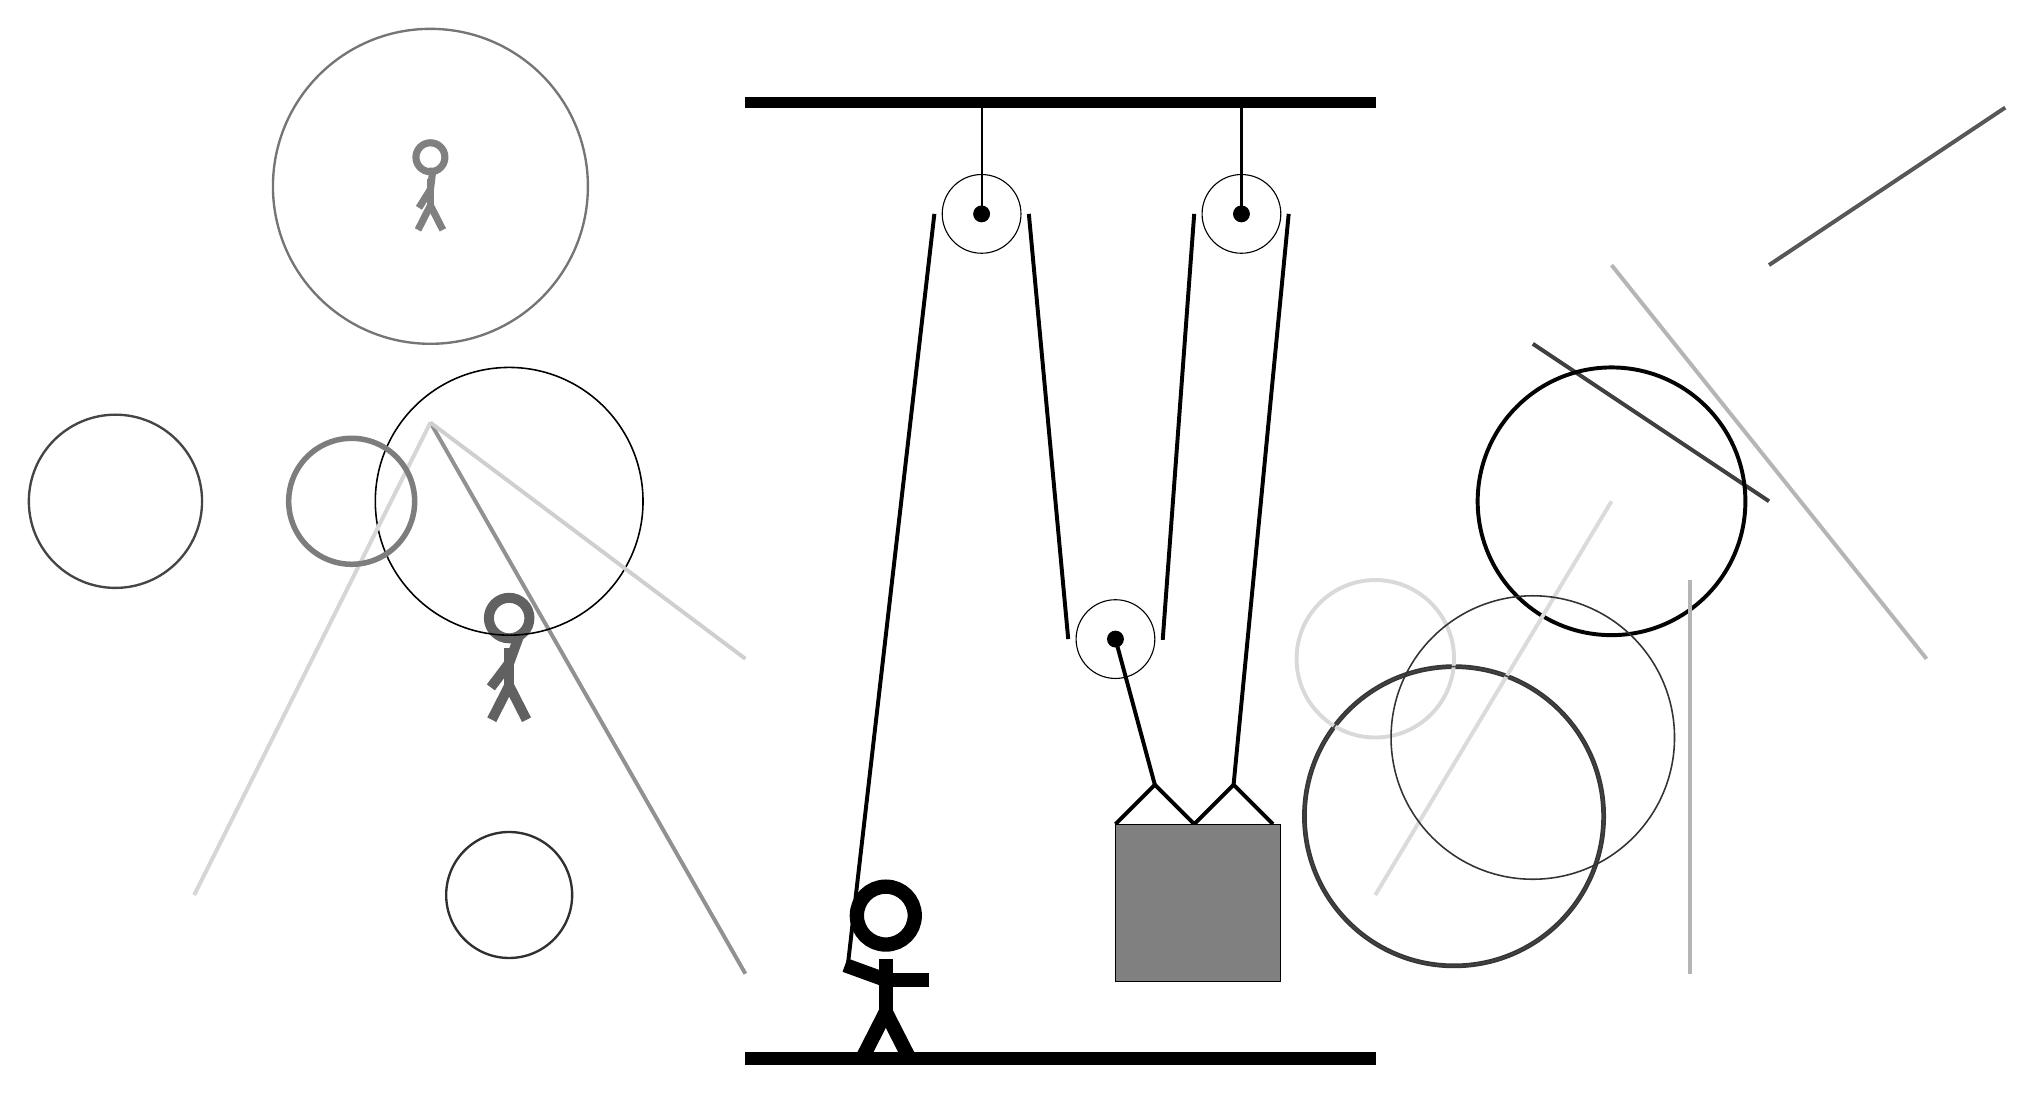
\begin{tikzpicture}
			%%%%% START %%%%%
			
			\draw[fill=black] (-2, 9) rectangle (6, 9.125);
			
			\draw (1, 7.65) circle (0.5);
			\draw[fill=black] (1, 7.65) circle (0.1);
			\draw[thick] (1, 7.65) -- (1, 9);
			
			\draw (4.3, 7.65) circle (0.5);
			\draw[fill=black] (4.3, 7.65) circle (0.1);
			\draw[thick] (4.3, 7.65) -- (4.3, 9);
			
			\draw [line width=0.3mm, color=black!73](-10, 4) circle (1.1);
			
			\node[line width=0.7mm, color=black!62] at (-5, 2) {\Strichmaxerl[7][53][70]};
			\draw[line width=0.5mm, color=black!75](11, 4) -- (8, 6);
			\draw [line width=0.6mm, color=black!79](7, 0) circle (1.9);
			\draw[line width=0.5mm, color=black!43](-2, -2) -- (-6, 5);
			
			\draw [line width=0.2mm, color=black!100](-5, 4) circle (1.7);
			
			\draw [line width=0.5mm, color=black!99](9, 4) circle (1.7);
			
			\draw[line width=0.5mm, color=black!16](-6, 5) -- (-9, -1);
			\draw[line width=0.5mm, color=black!29](10, -2) -- (10, 3);
			\draw [line width=0.6mm, color=black!48](-5, 5) circle (0.0);
			\draw[line width=0.5mm, color=black!66](11, 7) -- (14, 9);
			
			\draw[line width=0.5mm, color=black!19](-6, 5) -- (-2, 2);
			\draw [line width=0.3mm, color=black!54](-6, 8) circle (2.0);
			\draw[line width=0.5mm, color=black!29](9, 7) -- (13, 2);
			\node[line width=0.6mm, color=black!50] at (-6, 8) {\Strichmaxerl[5][58][83]};
			\draw[line width=0.5mm, color=black!14](6, -1) -- (9, 4);
			
			\draw [line width=0.5mm, color=black!15](6, 2) circle (1.0);
			
			\draw [line width=0.2mm, color=black!74](7, 0) circle (1.9);
			\draw [line width=0.3mm, color=black!81](-5, -1) circle (0.8);
			
			\draw [line width=0.2mm, color=black!80](8, 1) circle (1.8);
			\draw [line width=0.7mm, color=black!51](-7, 4) circle (0.8);
			
			
			\draw (2.7, 2.25) circle (0.5);
			\draw[fill=black] (2.7, 2.25) circle (0.1);
			
			\draw[line width=0.5mm]  (2.7, -0.1) -- (3.2, 0.4) -- (3.7, -0.1) -- (4.2, 0.4) -- (4.7, -0.1);
			\draw[fill=black!50] (2.7, -0.1) rectangle (4.8, -2.1);
			
			\draw[line width=0.5mm](-0.7, -1.9) -- (0.4, 7.65);
			\centerarc[line width=0.5mm](1, 7.65)(0:180:0.6);
			\draw[line width=0.5mm](1.6, 7.65) -- (2.1, 2.25);
			\centerarc[line width=0.5mm](2.7, 2.25)(180:370:0.6);
			\draw[line width=0.5mm] (3.3, 2.24) -- (3.7, 7.65);
			\centerarc[line width=0.5mm](4.3, 7.65)(0:180:0.6);
			\draw[line width=0.5mm](4.2, 0.4) -- (4.9, 7.65);
			\draw[line width=0.5mm] (3.2, 0.4) -- (2.7, 2.25);
			
			\node at (-0.2, -2) {\Strichmaxerl[10][-20][0]};
			
			\draw[fill=black] (-2, -3) rectangle (6, -3.15);
			
			%%%%% END %%%%%
		\end{tikzpicture}
	\end{figure}	
\end{document}